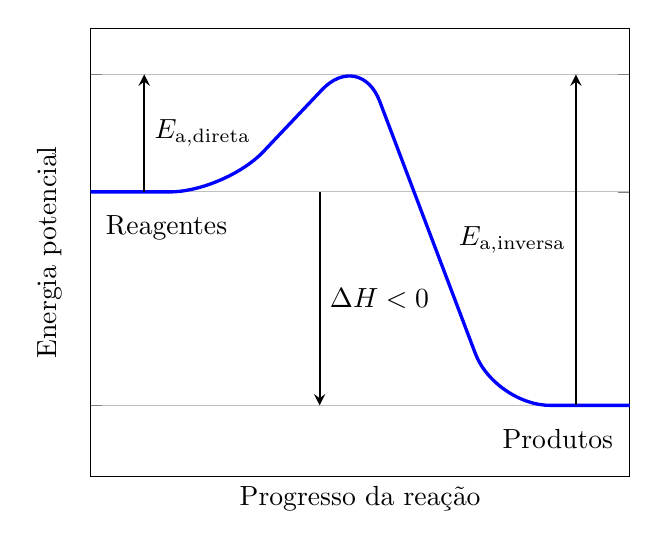
\begin{tikzpicture}
    \begin{axis}
        [
            grid = major,
            ylabel = {Energia potencial},
            xlabel = {Progresso da reação},
            xmin = 0, xmax = 4,
            ymin = -1, ymax = 5.3,
            xtick = \empty,
            ytick = {0, 3, 4.65},
            yticklabels = {},
        ]
        \draw [draw=blue, very thick, rounded corners=2em]
            (axis cs: 0, 3) -- 
            (axis cs: 1, 3) -- 
            (axis cs: 2, 5) -- 
            (axis cs: 3, 0) --
            (axis cs: 4, 0);
        \draw [ draw=black, thick, -stealth ]
            (axis cs: 0.4, 3.0) -- node [right] {$E_\mathrm{a, direta}$}
            (axis cs: 0.4, 4.65);
        \draw [ draw=black, thick, -stealth ]
            (axis cs: 3.6, 0.0) -- node [left] {$E_\mathrm{a, inversa}$}
            (axis cs: 3.6, 4.65);
        \draw [ draw=black, thick, -stealth ]
            (axis cs: 1.7, 3.0) -- node [right] {$\Delta H < 0$}
            (axis cs: 1.7, 0.0);
        \node [ below, align=center ] at (axis cs:0.6,2.8) 
            { Reagentes };
        \node [ below, align=center ] at (axis cs:3.5,-0.2) 
            { Produtos  };
     \end{axis}
 \end{tikzpicture}